\section{Digital Signature}
\label{sec:S3_digsign}

A digital signature is a mathematical technique used to validate the authenticity and integrity of a message, software or digital document.
The digital equivalent of a handwritten signature or stamped seal, but offering far more inherent security, a digital signature is intended to solve the problem of tampering and impersonation in digital communications. Digital signatures can provide the added assurances of evidence to origin, identity and status of an electronic document, transaction or message, as well as acknowledging informed consent by the signer.

\subsection{How digital signatures work}
\label{subsec:dgsign_work}

Digital signatures are based on public key cryptography, also known as asymmetric cryptography. Using a public key algorithm such as RSA, one can generate two keys that are mathematically linked: one private and one public. To create a digital signature, signing software (such as an email program) creates a one-way hash of the electronic data to be signed. The private key is then used to encrypt the hash. The encrypted hash, along with other information, such as the hashing algorithm, is the digital signature. The reason for encrypting the hash instead of the entire message or document is that a hash function can convert an arbitrary input into a fixed length value, which is usually much shorter. This saves time since hashing is much faster than signing.

The value of the hash is unique to the hashed data. Any change in the data, even changing or deleting a single character, results in a different value. This attribute enables others to validate the integrity of the data by using the signer's public key to decrypt the hash. If the decrypted hash matches a second computed hash of the same data, it proves that the data hasn't changed since it was signed. If the two hashes don't match, the data has either been tampered with in some way (integrity) or the signature was created with a private key that doesn't correspond to the public key presented by the signer (authentication). \cite{digsign}


\begin {figure}[h]
\graphicspath{{images/chapter_s3/}}
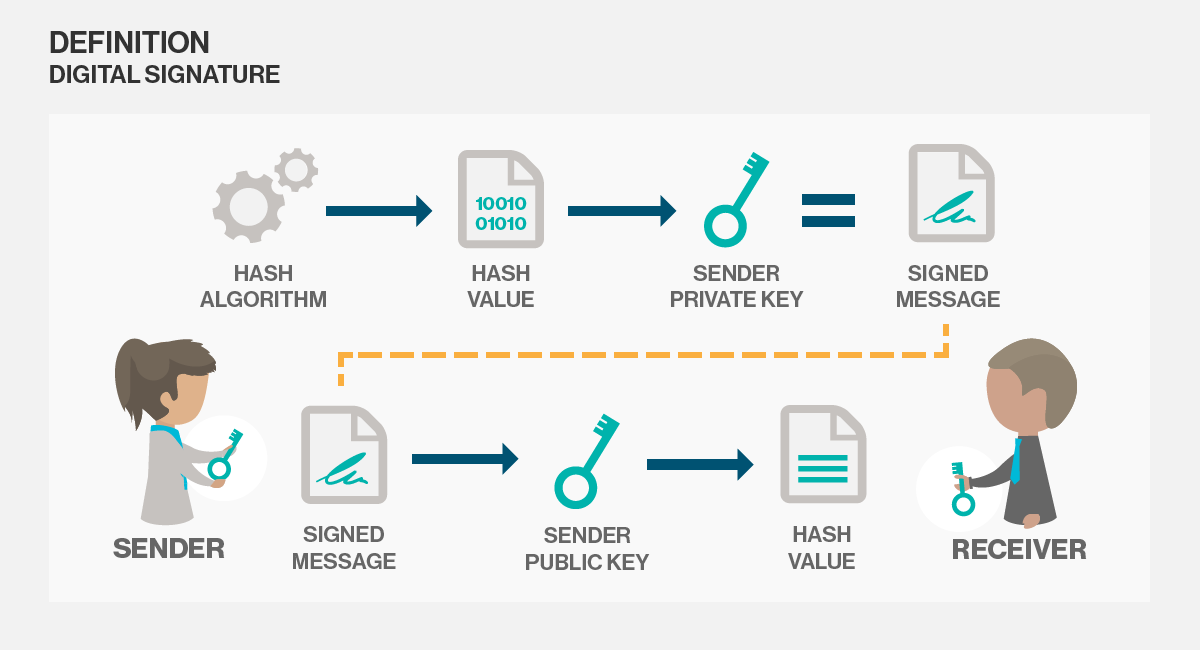
\includegraphics[width=\textwidth]{digsign}
\caption{Digital Signature Process}
\end {figure}

